Many observed phenomena are conspicuously absent in the SM, confirming that while self-consistent, the SM is ultimately an incomplete theory. The gravitational force; the matter composition of the universe (including dark matter and dark energy); the matter-antimatter asymmetry in the universe; and massive, oscillating neutrinos, to name a few, all lack any prediction in the SM. Attempts to model these phenomena within the paradigm of QFT and merge them with the SM are often called extensions to the SM or beyond the SM theories. Some extensions to the SM, such as Grand Unification~\cite{gut1}\cite{gut2}, Technicolor~\cite{techni1}\cite{techni2}\cite{techni3}, composite models, and Supersymmetry~\cite{superstring}, require a new boson that would uniquely carry both baryon number $B$ and lepton number $L$, generically called a leptoquark (symbolically, \LQ). Such a boson would mediate quark-lepton transitions and answer many of the questions left in the SM, such as the remarkable symmetry of the quark and lepton generations.

\subsection{Models} \label{sec:LQModels}


Leptoquarks can be scalar (spin 0) or vector (spin 1) bosons, are color-triplets under \SUthreeC, carry fractional electric charge and weak isospin. Listed in Table~\ref{tab:LQModels} are the possible quantum numbers a leptoquark may take assuming dimensionless couplings to SM fermions and invariance under the gauge group of the SM. The first two columns list the spin and fermion quantum numbers, followed by the QCD and weak isospin representations, the weak hypercharge, and the allowed couplings to chiral SM fermions (color indices, flavor indices, and charge conjugates have been supressed). As the right-most column of Table~\ref{tab:LQModels} shows, leptoquarks may couple to only right-chiral fermions or left-chiral fermions, called chiral leptoquarks, or one left-chiral and one right-chiral fermion, called non-chiral leptoquarks. The allowed lepton and quark generations have historically been constrained to the same generation, motived by experimental limits placed on rare processes like proton decay, and FCNCs~\cite{FCNC}. However, as detailed in Section~\ref{sec:ExperimentalMotivation}, allowing intergenerational mixing can provide an explaination for phenomena like the flavor anomalies and muon magnetic moment anomaly. 

For a given leptoquark model there are also a set of free parameters, which include the mass \MLQ the Yukawa coupling at the leptoquark-quark-lepton vertex $\lambda$, and the decay branching fraction into a charged lepton $\beta$ (with $\beta-1$ the branching fraction into a neutrino). Specific to vector leptoquark models are two additional parameters $\lambda_{\text{G}}$ and $\kappa_{\text{G}}$ that correspond to the couplings of leptoquarks to SM gauge bosons at the \HepProcess{\Pgluon\LQ} and \HepProcess{\Pgluon\Pgluon\LQ} vertices. The LHC is capable of both single- and pair-production of leptoquarks through large QCD cross sections, as shown in Figs.~\ref{fig:LQsingleprod} and~\ref{fig:LQpairprod}. 

\begin{table}[H]
    \begin{center}
        \caption{List of quantum numbers and allowed couplings to quarks/leptons for different leptoquark models.}
        \begin{tabular}{cccccl}
            \hline \hline
            Spin    & $3B+L$    & \SUthreeC                                 & \SUtwoW   & \UoneY        & Allowed coupling \\ \hline
            \num{0} & \num{-2}  & \num[parse-numbers=false]{\overline{3}}   & \num{1}   & \num{1/3}     & $\antispinor{\Pquark}{L}{c}\spinor{\Plepton}{L}{}$ or $\antispinor{\Pup}{R}{c}\spinor{\Pe}{R}{}$ \\ 
            \num{0} & \num{-2}  & \num[parse-numbers=false]{\overline{3}}   & \num{1}   & \num{4/3}     & $\antispinor{\Pdown}{R}{c}\spinor{\Pe}{R}{}$ \\ 
            \num{0} & \num{-2}  & \num[parse-numbers=false]{\overline{3}}   & \num{3}   & \num{1/3}     & $\antispinor{\Pquark}{L}{c}\spinor{\Plepton}{L}{}$ \\ 
            \num{1} & \num{-2}  & \num[parse-numbers=false]{\overline{3}}   & \num{2}   & \num{5/6}     & $\antispinor{\Pquark}{L}{c}\gammamu\spinor{\Pe}{R}{}$ or $\antispinor{\Pdown}{R}{c}\gammamu\spinor{\Plepton}{L}{}$ \\ 
            \num{1} & \num{-2}  & \num[parse-numbers=false]{\overline{3}}   & \num{2}   & \num{-1/6}    & $\antispinor{\Pup}{R}{c}\gammamu\spinor{\Plepton}{L}{}$ \\ 
            \num{0} & \num{0}   & \num{3}                                   & \num{2}   & \num{7/6}     & $\antispinor{\Pquark}{L}{}\spinor{\Pe}{R}{}$ or $\antispinor{\Pup}{R}{}\spinor{\Plepton}{L}{}$ \\ 
            \num{0} & \num{0}   & \num{3}                                   & \num{2}   & \num{1/6}     & $\antispinor{\Pdown}{R}{}\spinor{\Plepton}{L}{}$ \\ 
            \num{1} & \num{0}   & \num{3}                                   & \num{1}   & \num{2/3}     & $\antispinor{\Pquark}{L}{}\gammamu\spinor{\Plepton}{L}{}$ or $\antispinor{\Pdown}{R}{}\gammamu\spinor{\Pe}{R}{}$ \\ 
            \num{1} & \num{0}   & \num{3}                                   & \num{1}   & \num{5/3}     & $\antispinor{\Pup}{R}{}\gammamu\spinor{\Pe}{R}{}$ \\ 
            \num{1} & \num{0}   & \num{3}                                   & \num{3}   & \num{2/3}     & $\antispinor{\Pquark}{L}{}\gammamu\spinor{\Plepton}{L}{}$ \\ \hline \hline
        \end{tabular}
        \label{tab:LQModels}
    \end{center}
\end{table}

\begin{figure}[H]
    \centering
    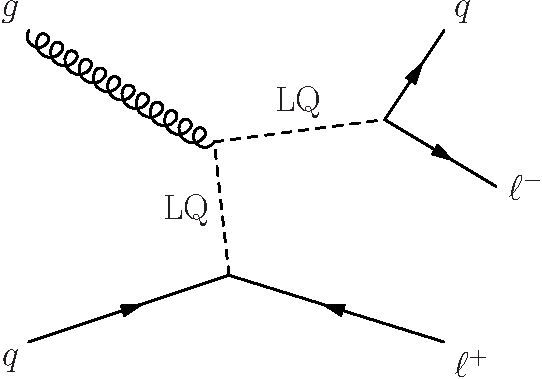
\includegraphics[width=0.3\textwidth]{Images/Theory/SingleLQProdT1.pdf}\hspace{0.1\textwidth}
    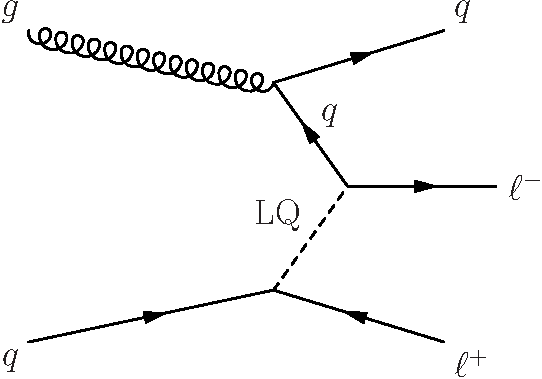
\includegraphics[width=0.3\textwidth]{Images/Theory/SingleLQProdT2.pdf}\vspace{0.05\textwidth}
    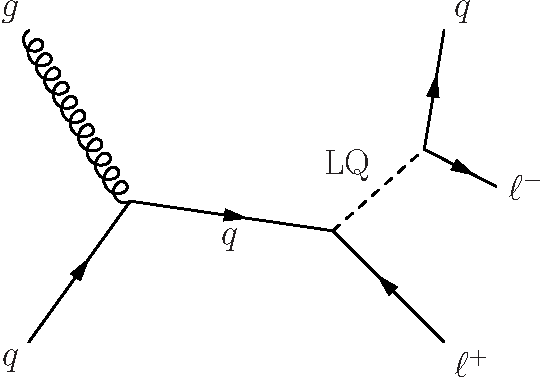
\includegraphics[width=0.3\textwidth]{Images/Theory/SingleLQProdS1.pdf}\vspace{0.05\textwidth}
    \caption{Production mechanisms of single leptoquarks at the LHC. Clockwise from top left: a t-channel processes that results in a resonant \HepProcess{\Pquark\Plepton} pair and a non-resonant \Plepton, a t-channel processes resulting in a non-resonant \HepProcess{\Plepton\Plepton\Pquark} final state, and an t-channel process resulting in a resonant \HepProcess{\Pquark\Plepton} pair and a non-resonant \Plepton.}
    \label{fig:LQsingleprod}
\end{figure}

\begin{figure}[H]
    \centering
    \includegraphics[width=0.3\textwidth]{Images/Theory/LQLQProduction_1.pdf}\hspace{0.1\textwidth}
    \includegraphics[width=0.3\textwidth]{Images/Theory/LQLQProduction_3.pdf}\vspace{0.05\textwidth}
    \includegraphics[width=0.3\textwidth]{Images/Theory/LQLQProduction_2.pdf}\hspace{0.1\textwidth}
    \includegraphics[width=0.3\textwidth]{Images/Theory/LQLQProduction_4.pdf}\vspace{0.05\textwidth}
    \caption{Production mechanisms of \HepProcess{\LQ\LQbar} pairs at the LHC. Clockwise from top-left: s-channel gluon-gluon fusion, gluon-gluon four-point interaction, t-channel gluon-gluon interaction via leptoquark exchange, and s-channel quark-antiquark annihilation.}
    \label{fig:LQpairprod}
\end{figure}

\subsection{Experimental motivation} \label{sec:ExperimentalMotivation}
% Flavor anomalies (LHCb)

The SM assumes that the weak gauge bosons couple to each lepton flavor identically (or close to it), a phenomenon called lepton flavor universality. Tests of lepton flavor universality can be performed by studying flavor-changing neutral current (FCNC) transitions, such as when a bottom quark transforms into strange quark in the decay: $B^+\rightarrow K^+\ell^+\ell^-$. As FCNC are suppressed at tree-level in the SM, occuring only via higher order electroweak processes (as shown in the left-hand diagram of Fig.~\ref{fig:FCNC}), these decays are a powerful probe into new physics. Measurements by the LHCb, BaBar, and Belle collaborations of observables such as $R_K$, $R_{K*}$, $R_D$, and $R_{D*}$---the decay branching fractions of $B$ mesons into an electron-positron pair over a muon-antimuon pair---hint at a possible violation of lepton flavor universality. Combining the flavor anomalies from each collaboration in $R_K^*$ (Fig.~\ref{fig:FlavorAnomalies}, left) yields tension between experiment and the SM at 2 standard deviations~\cite{LHCb1}, and for $R_K$ (Fig.~\ref{fig:FlavorAnomalies}, right) up to 3.1 standard deviations~\cite{LHCb2}. Leptoquarks coupling to muons and bottom quarks are prime candidates to explain these flavor anomalies at tree-level, as shown in the right-hand diagram of Fig.~\ref{fig:FCNC}.

\begin{figure}[H]
    \centering
    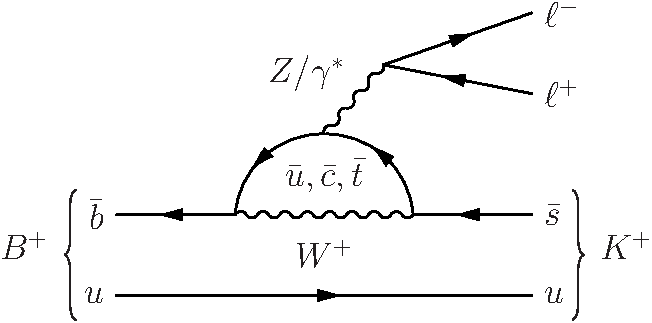
\includegraphics[width=0.4\textwidth]{Images/BplusDecayFCNC.pdf}\hspace{0.1\textwidth}
    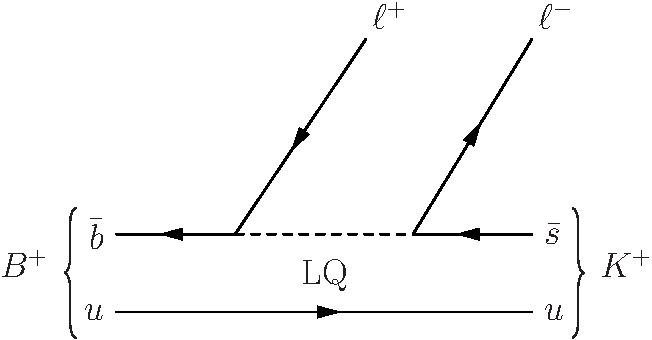
\includegraphics[width=0.4\textwidth]{Images/BplusDecayLQ.pdf}
    \caption{The decay of a charged $B$ meson into a charged kaon and a pair of opposite-sign charged leptons. Left: An example of a loop diagram FCNC process in the SM that is strongly suppressed. Right: A tree-level FCNC solution with a leptoquark mediating the transition.}
    \label{fig:FCNC}
\end{figure}

\begin{figure}[H]
    \centering
    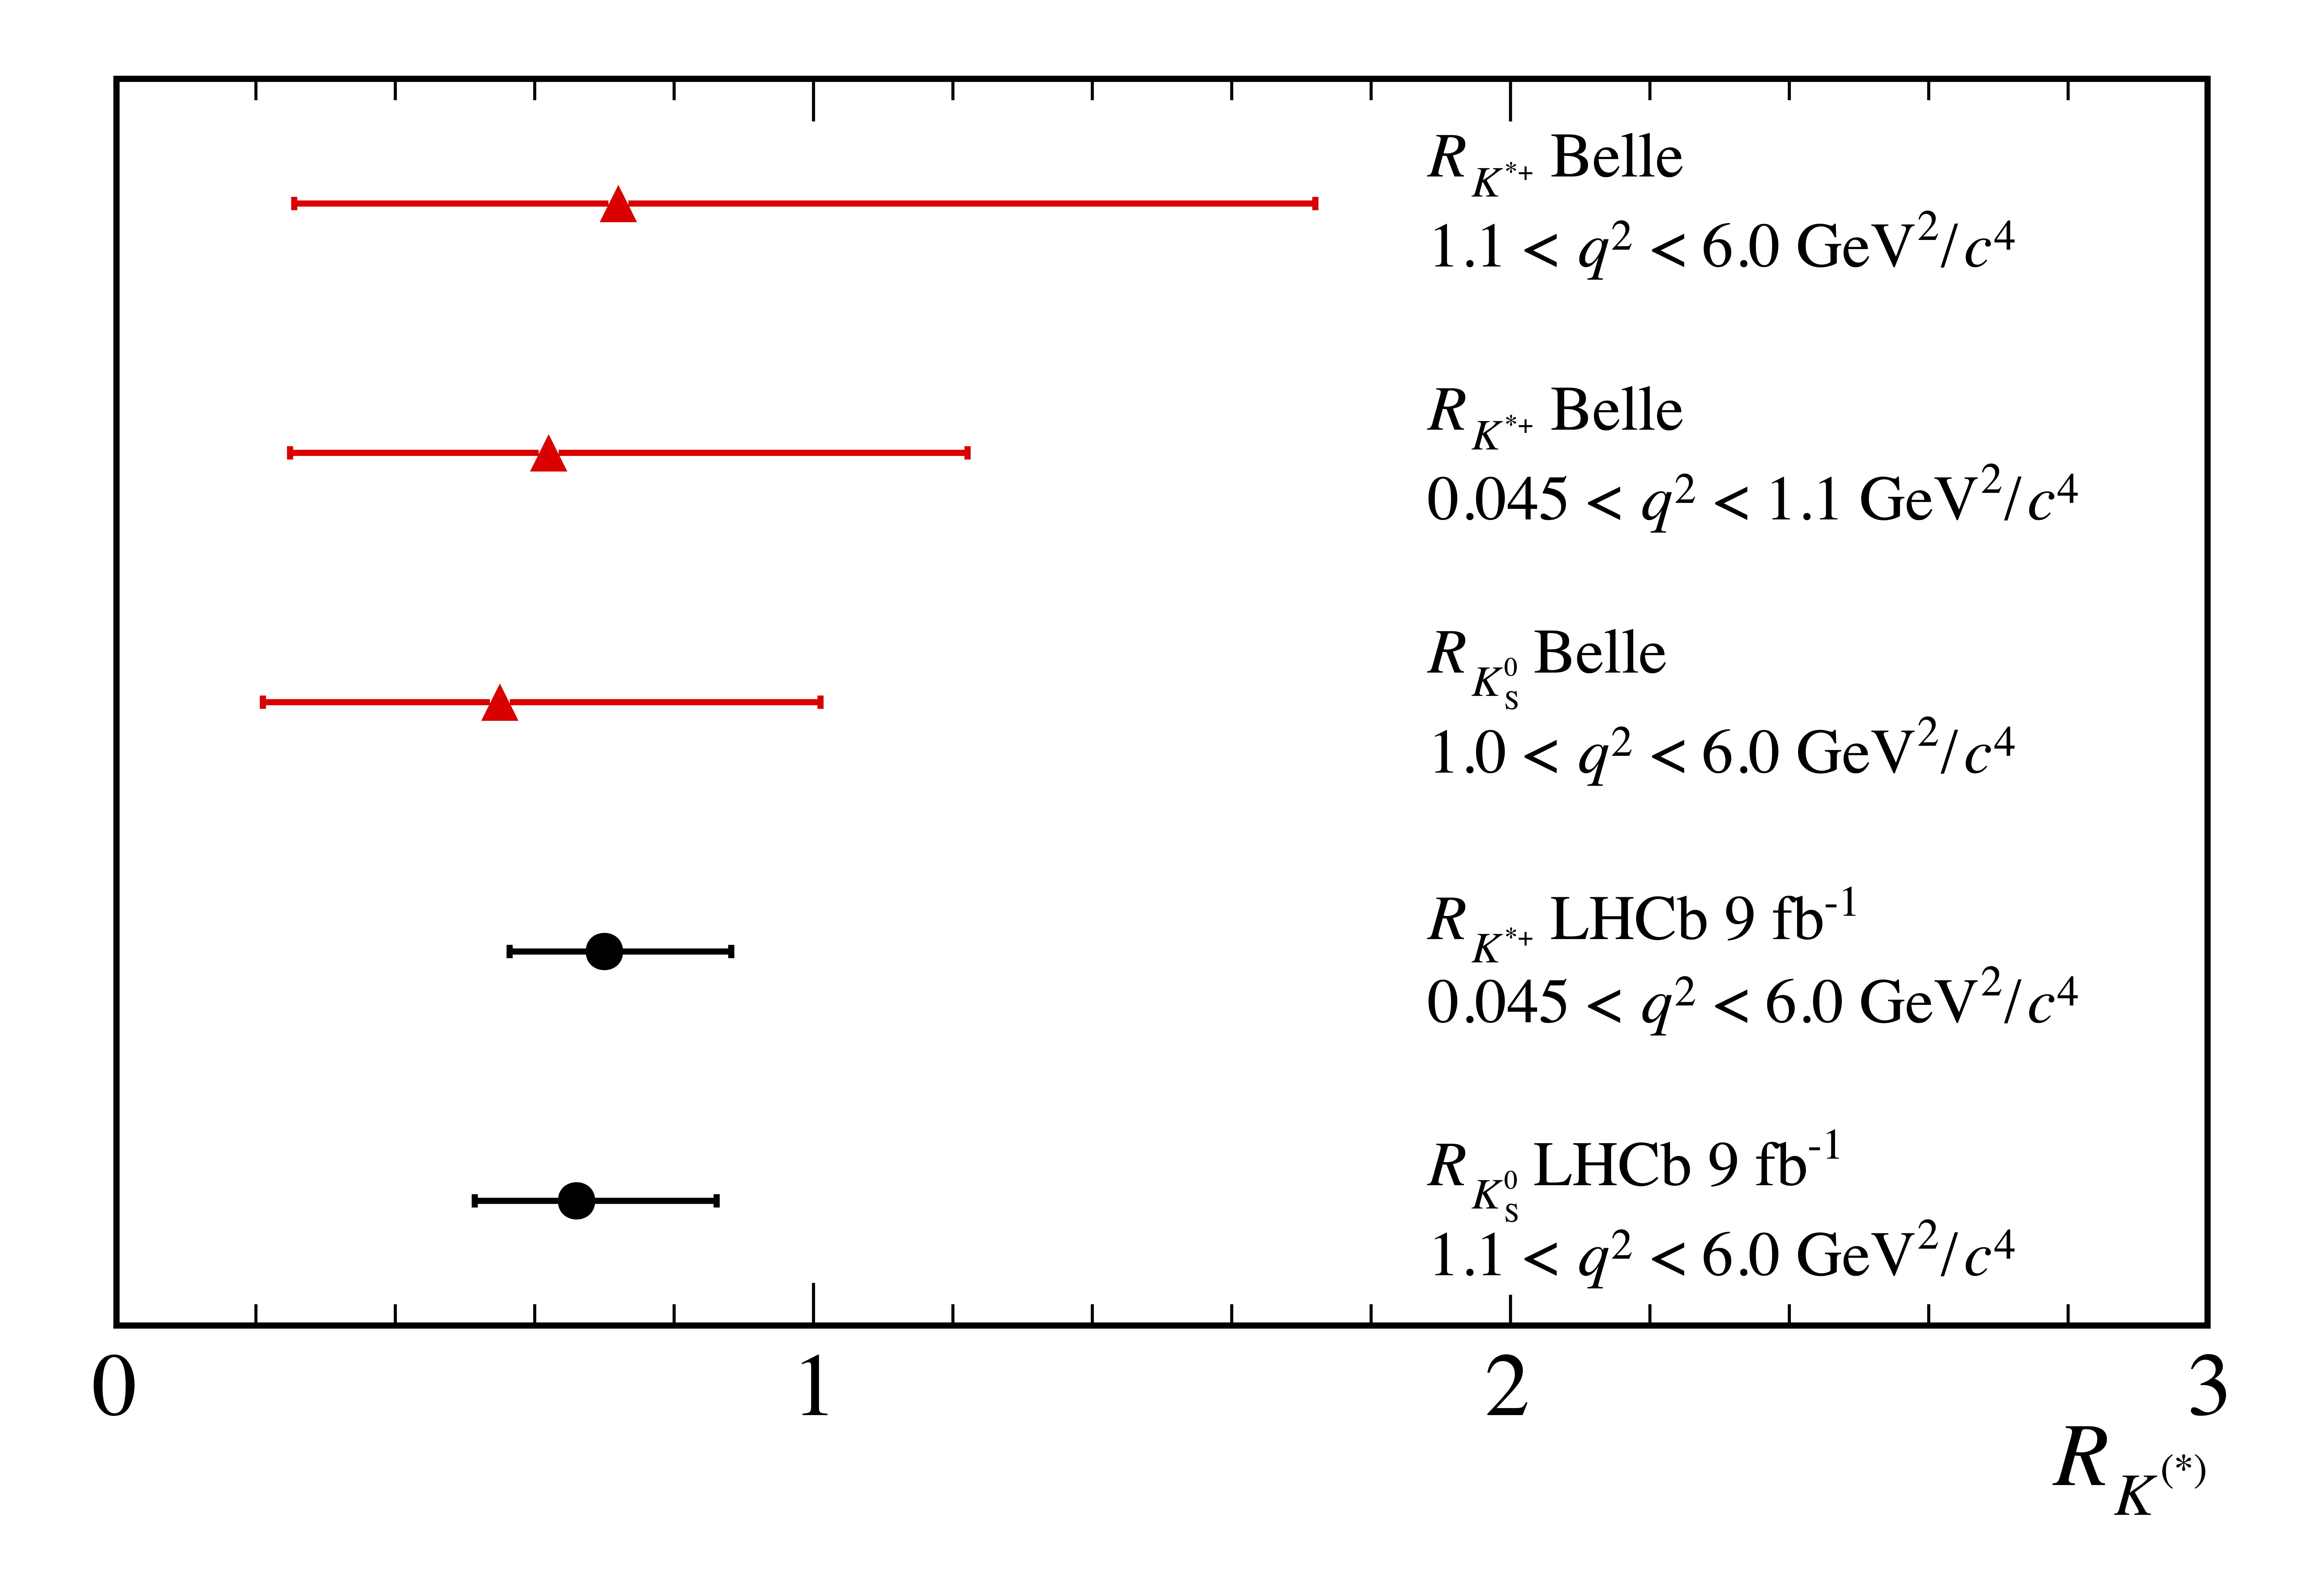
\includegraphics[width=0.49\textwidth]{Images/LHCbBelle.png}
    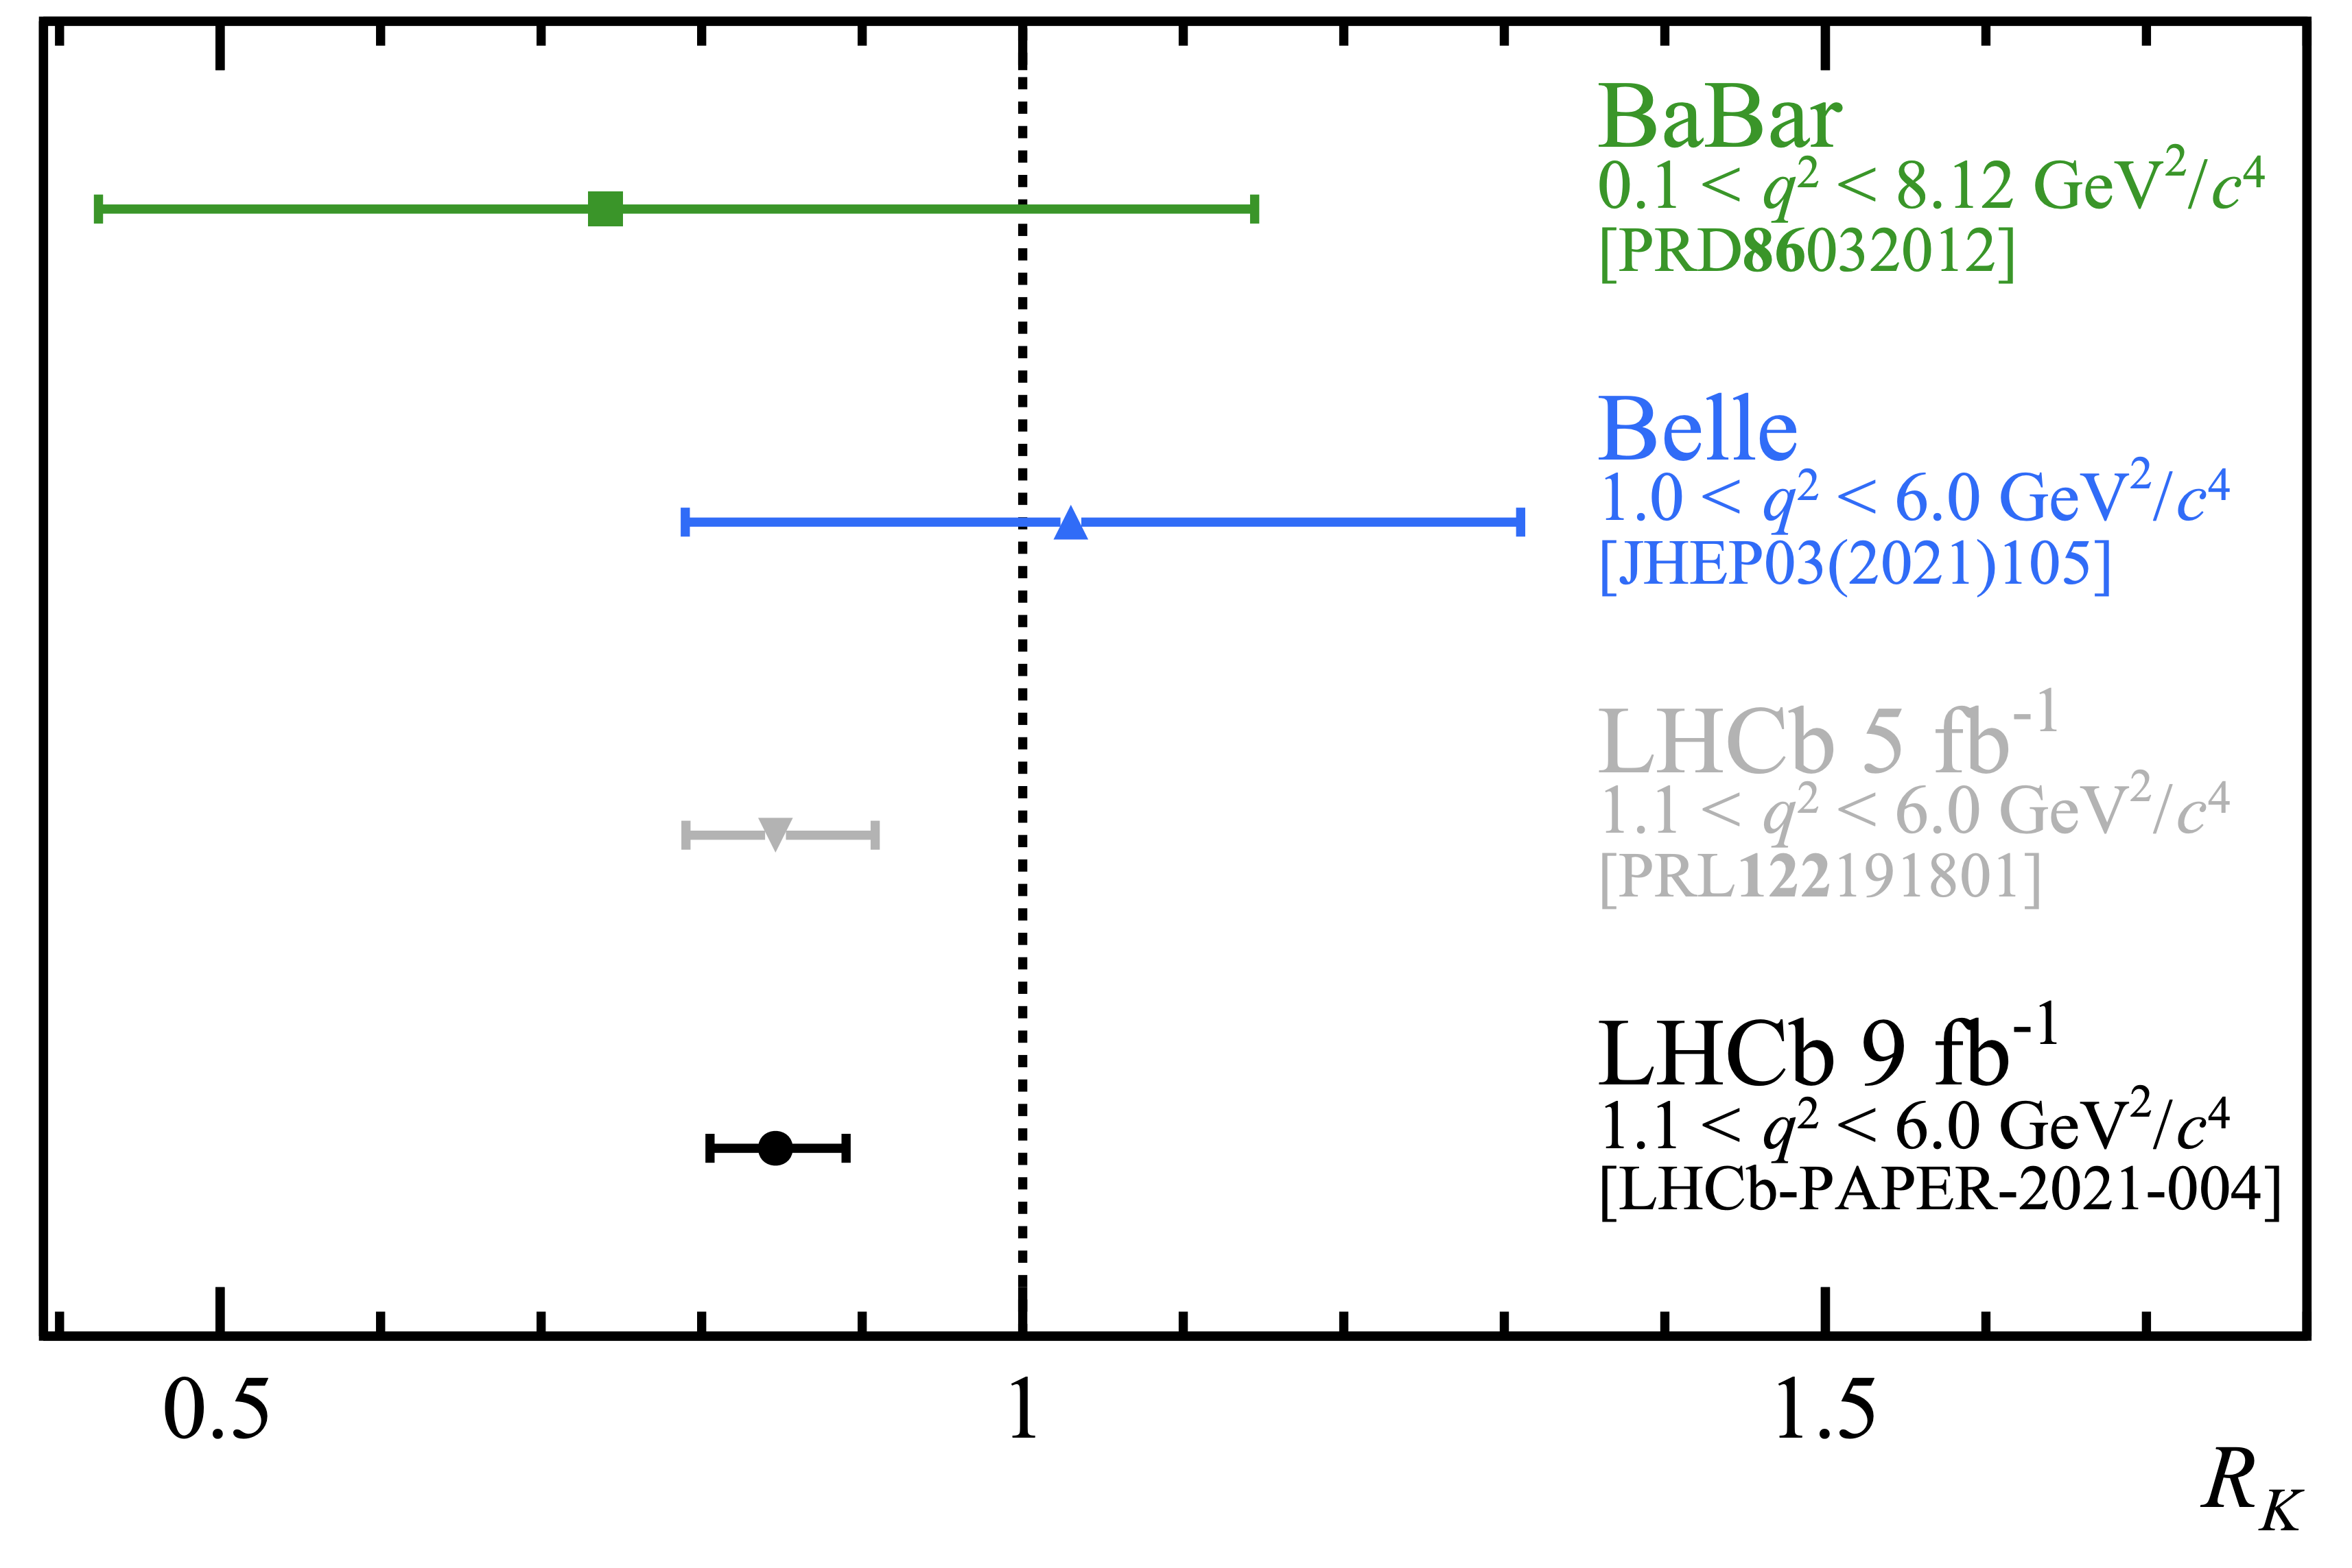
\includegraphics[width=0.49\textwidth]{Images/RKmeasurements.png}
    \caption{Left: A comparison of $R_{K*}$ measurements by the Belle and LHCb collaborations for several bands of the dilepton invariant mass squared $q^2$. Right: A comparison of $R_K$ measurements (combining $B^+\rightarrow K^+\ell^+\ell^-$ and $B^0\rightarrow K^0_s\ell^+\ell^-$ decays) by the BaBar, Belle, and LHCb collaborations for several bands of the dilepton invariant mass squared $q^2$.}
    \label{fig:FlavorAnomalies}
\end{figure}

% Muon magnetic moment anomaly (Muon g-2)

Another notable inconsistency between the SM prediction and experiment in which leptoquarks may play a role is the anomalous muon magentic dipole moment. The magnetic moment of the muon is defined as:

\begin{equation}
    \vec{\mu} = g_{\mu}\left(\frac{q}{2m_{\mu}}\right)\vec{s}
\end{equation}
where the factor $g_{\mu}$ as predicted by the Dirac equation is equal to 2. Considering a number of EM, EW, and QCD radiative corrections (a few example diagrams are shown in Fig.~\ref{fig:amu}, left), the SM value of $g_{\mu}$ is predicted with high precision to deviate from 2, encapsulated in the muon magnetic anomaly $a_{\mu} = (g_{\mu}-2)/2$. Recent calculations set the SM theoretical value $a_{\mu}(\mathrm{SM})=\num{116591810(43)e-11}$, a precision of 0.37 parts-per-million (ppm). Measurements of $a_{\mu}$ by the Muon $g-2$ experiment at Brookhaven National Laboratory (BNL) and Fermilab National Accelerator Laboratory (FNAL) found a combined experimental average of $a_{\mu}(\mathrm{Exp}) = \num{116592061(41)e-11}$, with an astonishing precision of 0.34 ppm~\cite{Muongminus2}, as shown in Fig.~\ref{fig:amuExp}. The difference between the theoretical prediction and the experimental average has a significance of 4.2 standard deviations. Introducing leptoquarks that couple to muons could explain the deviation form the SM, as seen in the diagram in Fig.~\ref{fig:amuLQ}.

\begin{figure}[H]
    \centering
    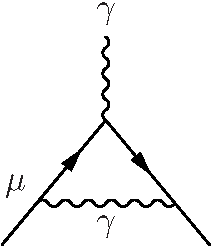
\includegraphics[width=0.2\textwidth]{Images/Muon_gminus2_photon.pdf}\hspace{0.05\textwidth}
    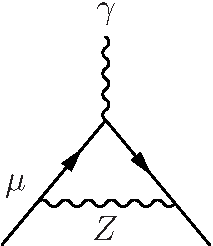
\includegraphics[width=0.2\textwidth]{Images/Muon_gminus2_Z.pdf}\hspace{0.05\textwidth}
    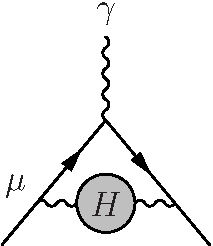
\includegraphics[width=0.2\textwidth]{Images/Muon_gminus2_Hadronic.pdf}\hspace{0.05\textwidth}
    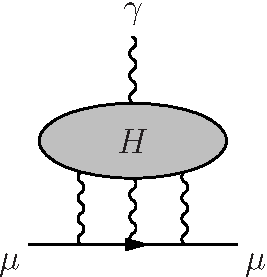
\includegraphics[width=0.2\textwidth]{Images/Muon_gminus2_Hadronic2.pdf}
    \caption{The Feynman diagrams of SM contributions to the muon anomaly. From left to right: the first-order QED and weak processes, leading-order hadronic vacuum polarization, and hadronic light-by-light contributions.}
    \label{fig:amu}
\end{figure}

\begin{figure}[H]
    \centering
    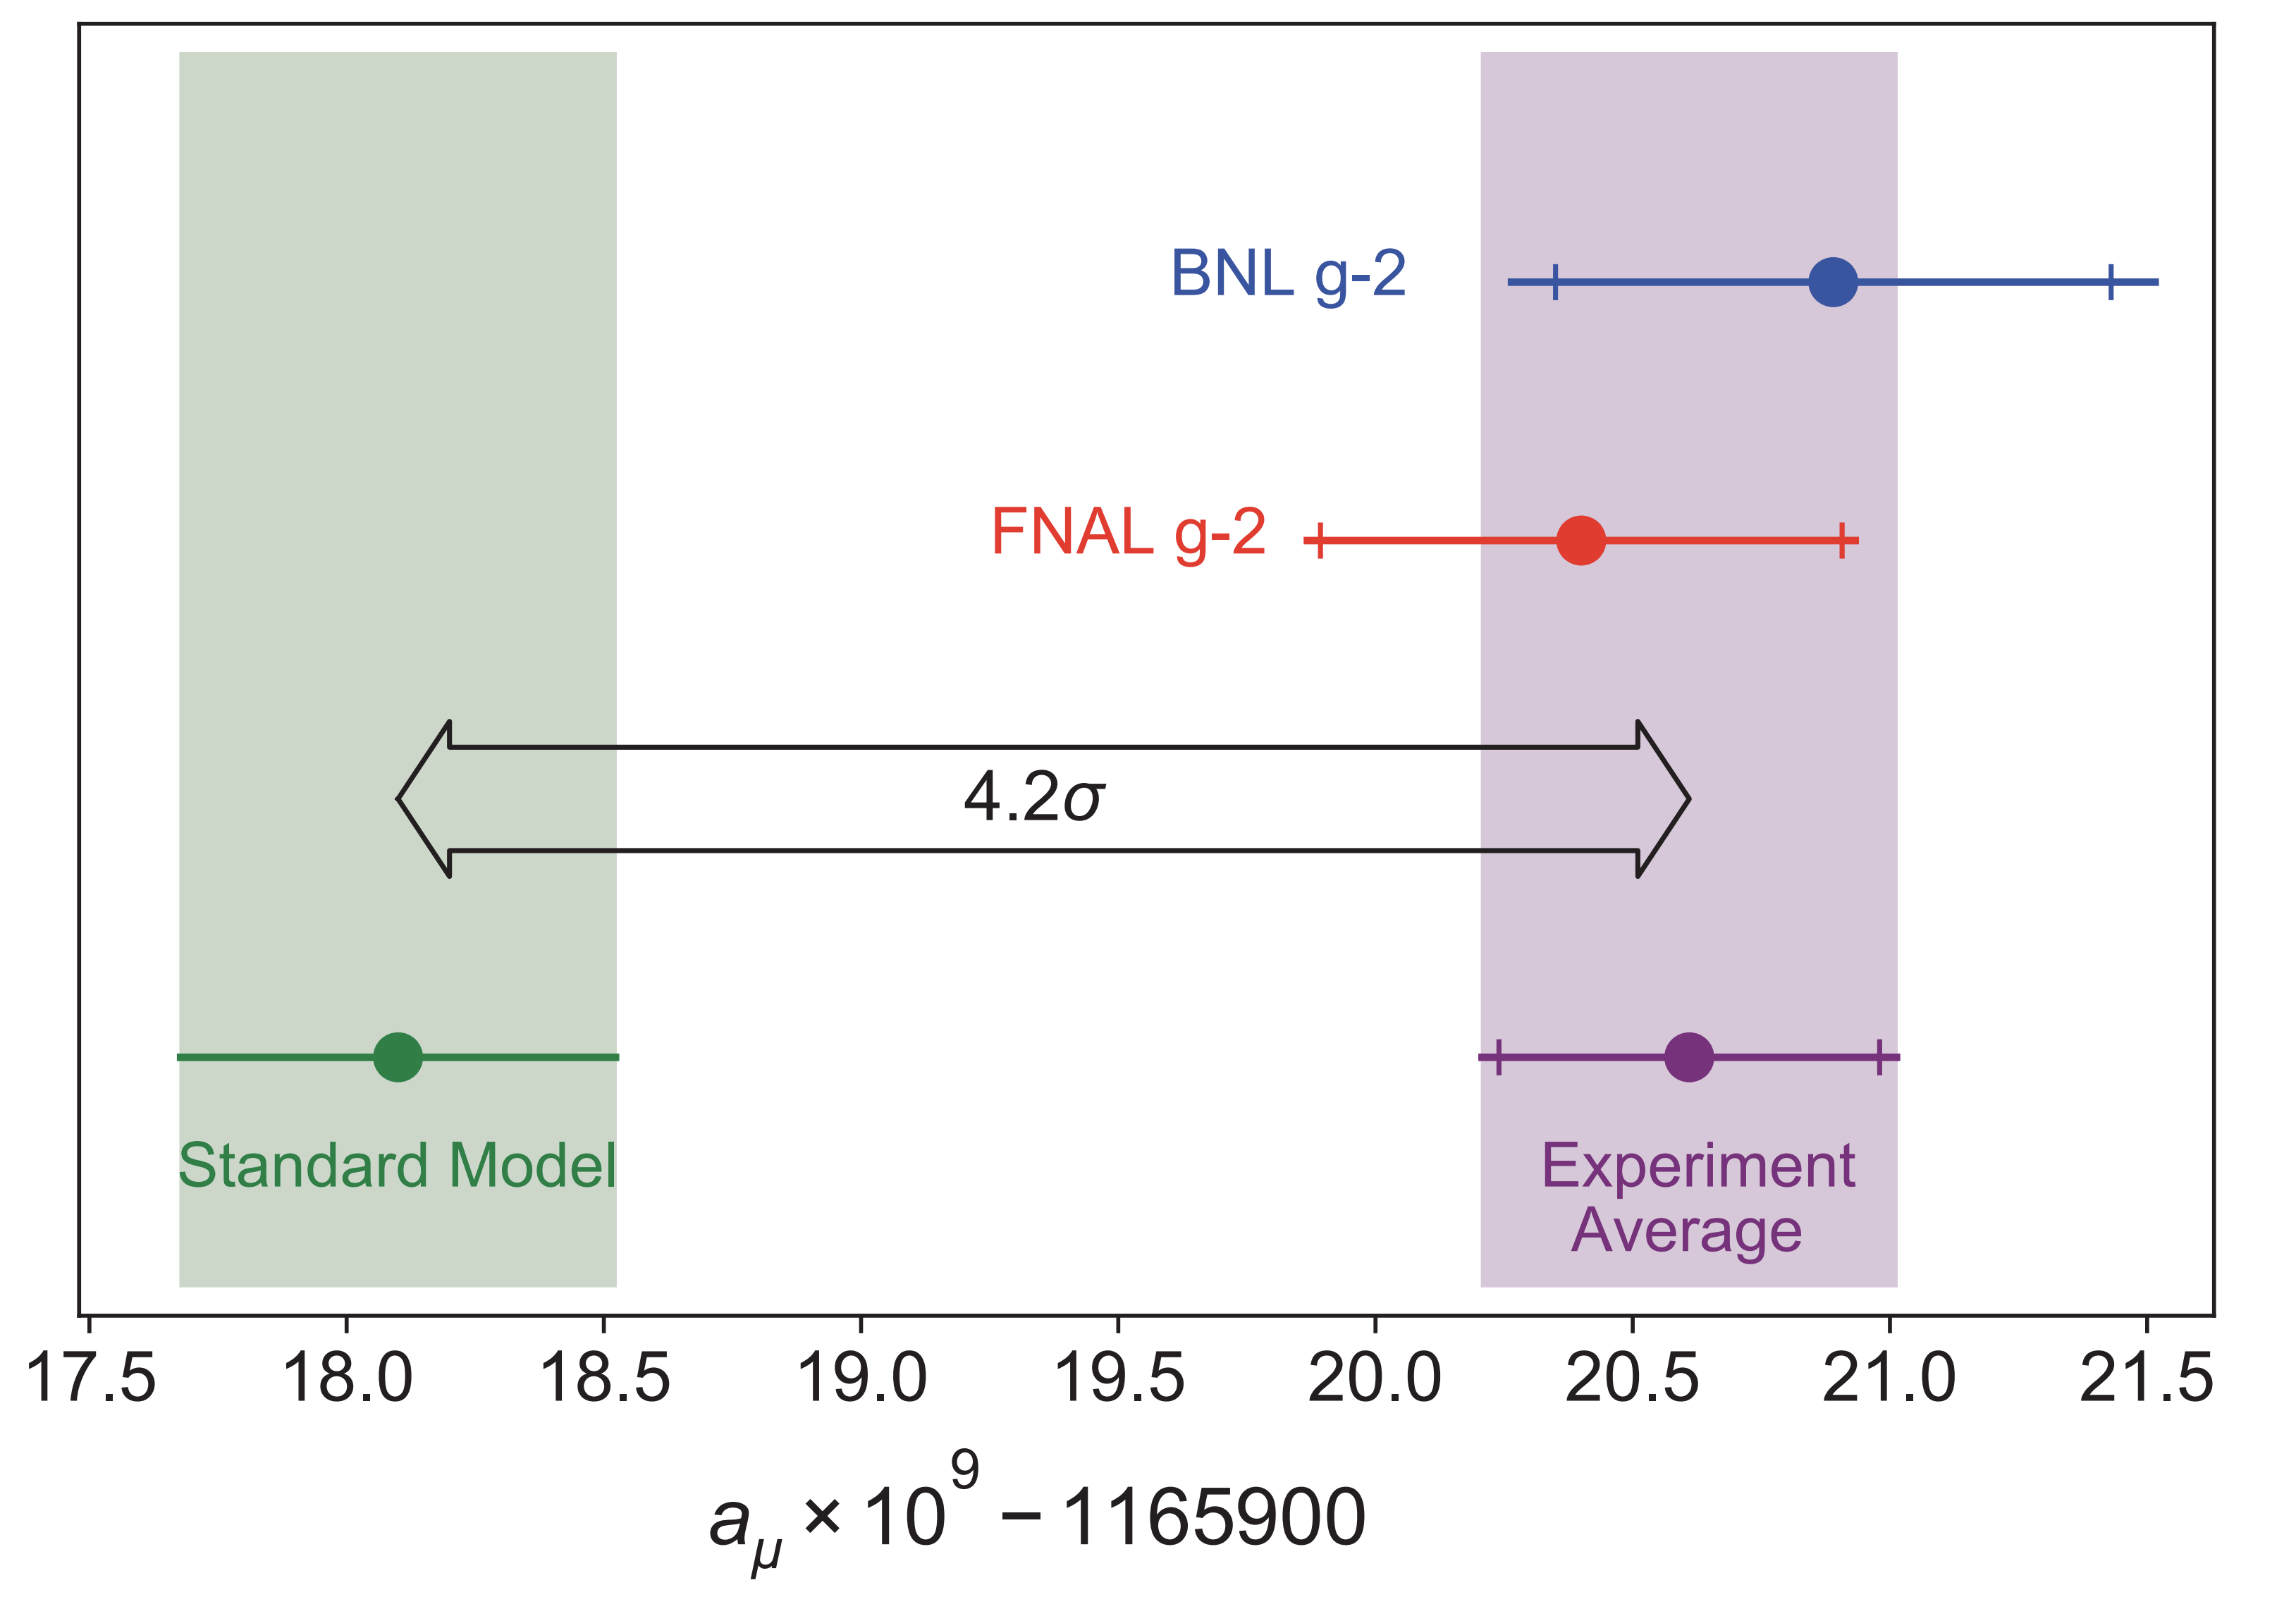
\includegraphics[width=0.7\textwidth]{Images/MuonAnomaly.png}
    \caption{A comparison of $a_\mu$ measured by BNL, FNAL, and the combined average beside the SM prediction.}
    \label{fig:amuExp}
\end{figure}

\begin{figure}[H]
    \centering
    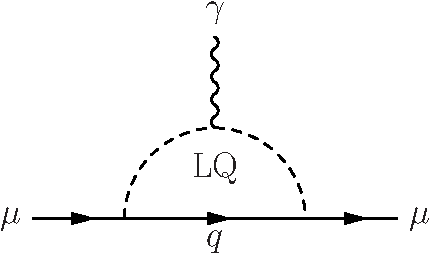
\includegraphics[width=0.5\textwidth]{Images/Muon_gminus2_LQ.pdf}
    \caption{A Feynman diagram of a leptoquark solution to the magnetic anomaly $a_{\mu}$.}
    \label{fig:amuLQ}
\end{figure}

\subsection{This search} \label{sec:ThisSearch}
The leptoquark search detailed in Chapter~\ref{chapter:LeptoquarkSearch} considers only pair-produced scalar leptoquarks that couple to a bottom quark and muon, but is otherwise model independent. These search parameters constrain $\lambda_G$ and $\kappa_G$ to zero, $\beta$ to unity, and keeps the search insensitive to $\lambda$, leaving $M_{\LQ}$ the only search variable. Previous limits on leptoquark masses~\cite{} motivate a mass scan of 30 points ranging from 300~GeV to 4000~GeV. This search is the first leptoquark search with muons in the final state to analyze the entire LHC Run II dataset collected by CMS and the first ever search for the process $\LQ\LQ\rightarrow\mu\mu bb$ by CMS.
